%
% fig-gebiet.tex
%
% (c) 2025 Prof Dr Andreas Müller
%
\begin{figure}
\centering
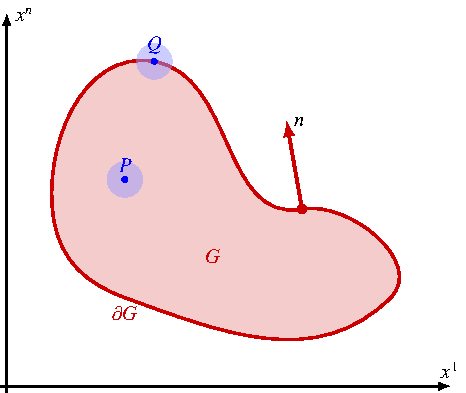
\includegraphics{chapters/080-feldgleichungen/images/gebiet.pdf}
\caption{Gebiet und Rand.
Der Punkt $P$ ist ein innerer Punkt des Gebietes, da es eine kleine
Umgebung gibt, die vollständig in $G$ enthalten ist.
Der Punkt $Q$ ist ein Randpunkt, $Q\in\partial G$, weil jede Umgebung
sowohl Punkte von $G$ wie auch von $\mathbb{R}^n\setminus G$ enthält.
Die Normale $n$ auf den Rand wird zur Definition der Neumann-Randbedingungen
verwendet.
\label{buch:feldgleichungen:loesungsverfahren:fig:gebiet}}
\end{figure}
